\documentclass[a4paper,12pt]{article}
\usepackage[colorlinks=true, linkcolor=blue, urlcolor=blue, citecolor=blue]{hyperref}
\usepackage{algorithm}
\usepackage{algpseudocode}
\usepackage[a4paper, left=1.5cm, right=1.5cm, top=2cm, bottom=2cm]{geometry}
\usepackage{float}
\usepackage[none]{hyphenat}
\usepackage{graphicx}
\usepackage{amsmath}
\usepackage{tikz}
\usetikzlibrary{shapes, arrows.meta, positioning}
\usepackage{tabularx}
\usepackage{titling}

\title{\Huge Paths and cycles enumeration methods in graphs --- GSoC 2025}
\author{Ziad Tarek}
\date{}

\begin{document}

\pretitle{%
    \begin{center}
    
\includegraphics[width=10cm]{logo_sagemath.png}\\[\bigskipamount]
}

\maketitle
\tableofcontents
\listofalgorithms
\newpage

\section{Personal}

\begin{itemize}
  \item Name: Ziad Tarek Abdelaziz
  \item Contact Information:
        \begin{itemize}
          \item Email: \href{mailto:ziad20037891@gmail.com}{ziad20037891@gmail.com}
          \item Discord: zezoo050
        \end{itemize}
  \item Github: \href{https://github.com/zezoo050}{zezoo050}
  \item Location/Timezone: Cairo --- Egypt (UTC/GMT +2 hours)
  \item University/Employment: Student at Faculty of Computer and Information Sciences
        at Ain Shams University
\end{itemize}


\section{Background}

% What are your technical skills, 
% education, experience, etc. 
% Especially make sure to explain with what level of 
% mathematics you are comfortable with and on what level you 
% would like to program.

\subsection{Education, Technical Background and experience}
I am currently a senior, set to graduate in a few months. Over the past few
years, I have studied various courses and gained experience in many areas. I
have mainly focused on competitive programming and have achieved several
successes:
\begin{itemize}
      \item Champion of
            \href{https://icpc.global/regionals/finder/ECPC-2025/standings}{ECPC 2024}
            (ICPC Egyptian Collegiate Programming Contest)
      \item Silver medalist with Rank 3 at
            \href{https://icpc.global/regionals/finder/ACPC-2025/standings}{ACPC 2024}
            (ICPC Africa \& Arab Collegiate Programming Championship)
      \item Qualified for the ICPC World Finals 2025 in Baku, Azerbaijan
      \item Finalist at the ICPC World Finals 2024 in Astana, Kazakhstan
\end{itemize}

You can view all my competitive programming achievements on my
\href{https://icpc.global/ICPCID/FRKWA0PTZMC8}{ICPCID}, or
\href{https://codeforces.com/profile/zezoo050}{Codeforces: zezoo050}.\\

I also joined \href{https://www.facebook.com/acmASCIS}{acmascis}, a competitive
programming community that trains and prepares students for contests. In my
junior year, I led the problem-setting and testing teams. We created and tested
problems not only for regional contests in Africa and the Arab region but also
for the community to help train students. I managed about 15 members, ensuring
that we met the community’s needs for problems. Additionally, I trained team
members so they could continue leading the community in the future.\\

Regarding mathematics, I am comfortable with the level needed to understand
algorithms and the math used in computer science. As part of my training for
competitive programming, I have studied various fields such as linear algebra,
discrete math, graph theory, and geometry.\\

For programming, I have experience at different levels. I have worked on many
projects, from building websites to developing low-level projects like database
engines and operating systems.\\

% Who are you? What makes you the best person to work on this particular project? Your personal motivation?

\subsection{About me \& motivation}
I have been interested in computer science since high school. When I started
college, people suggested I try competitive programming. As a naturally
competitive person, I found it enjoyable and learned a lot from it. After a
couple of years, I noticed improvements in my speed and problem-solving skills,
even for problems outside competitive programming. This training also made a
big difference in my ability to handle projects and my understanding to
theories. \\

My motivation for this project comes from two main sources. First, my passion
for graph theory drives me to explore its many applications. Second, I have a
strong desire to give back to the open source community. I have been using
Linux and other open source software for several years, and these resources
have helped me learn and grow. Now, I feel it is my turn to contribute. Google
summer of code is a very good opportunity to get into open source. I am still a
beginner and have a lot to learn, but I will do my best to contribute and
continue growing in this field.\\

% What platform and operating-system are you using on your computer? (SageMath development is done best on Linux, !MacOS, or Windows through WSL)
\subsection{Operating system \& Development environment}
I have been using Linux for almost four years and have gained a lot of
experience with it. Currently, my main operating system is Ubuntu.\\

% Are you or have you been engaged in other open-source projects?
\subsection{Open source contributions}
SageMath is my first open-source contribution. I have been using open-source
software as much as possible and have explored the code of multiple open-source
projects. However, my first direct engagement has been with SageMath. I was
able to build SageMath from source code and familiarized myself with the source
code. I was able to find a fix for an issue and opened a pull request
(\href{https://github.com/sagemath/sage/pull/39754}{\#39754}) and it got
approved. Additionally, reported a bug
(\href{https://github.com/sagemath/sage/issues/39756}{\#39756}).\\

% Do you code on your own pet projects?
\subsection{Pet projects}
I do code on my own pet projects from time to time when I get interested in
something, but currently I am more focused on GSoC and being able to contribute
to open source projects. Here are some of the projects that could be of an
interest:
\begin{itemize}
      \item \href{https://github.com/zezoo050/ImageEncryptCompress}{ImageEncryptCompress}: Compression and Decompression of images using Huffman tree, and also encryption and decryption of images.
      \item \href{https://github.com/zezoo050/spacechickensfmlgame}{spacechickensfmlgame}: space chicken game built using C++ and SFML.
      \item \href{https://github.com/zezoo050/GSoC25-SageMath-proposal}{GSoC25-SageMath-proposal}: I actually consider this proposal as one of my pet projects that I am proud of. 
      While I have been using $Latex$ for technical writing for competitive programming problems, I have never used it on such a scale as this proposal before.
\end{itemize}

% TODO: add this proposal as pet project

% Are you a SageMath user, how long have you known about/used SageMath?
\subsection{SageMath knowledge}
My knowledge of SageMath does not exceed a couple of months. I have been using
it for graph theory purposes, applying algorithms and visualizing graphs.



\section{Project}

\begin{itemize}
  \item \textbf{Title:} Paths and cycles enumeration methods in graphs
  \item \textbf{Length:} Medium (175 hours)
\end{itemize}

% Project Synopsis: A short description and summary of its aim and scope.
\subsection{Project Synopsis}
The project is aimed to add some functionalities related to graph theory in
SageMath. Specifically, it aims to add the following objectives:

\begin{itemize}
  \item Add a method for the enumeration of simple cycles in undirected graphs, as
        there is already an implemented method for directed graphs. Then extend these
        methods to support enumeration of cycles by increasing weight.
  \item Implement recent and more efficient methods for finding the k shortest simple
        paths in (un) weighted (di) graphs.
  \item Unify the input and output of these methods to ensure similar behaviors.
\end{itemize}

\subsection{Personal involvement}
% What is your personal involvement or relationship with your proposed project?
During my competitive programming experience, I was exposed to many areas of
mathematics, including graph theory, which I found especially interesting. I
became the team member with the most training and strength in graph theory on
my competitive programming team. When I saw this project idea, I felt it was
the perfect fit for me. I am confident that I have solved variations of the
problems in this project during my training and in official contests. In
addition, my experience in setting and testing problems has given me the skills
needed to work on graph theory challenges.

% Details: Describe all the details and explain modules or parts 
% of your whole project. Break down the whole project into 
% individual tasks - as good as possible - and describe deliverable 
% and quantifiable results for each of them. It also helps if you have 
% already discussed this with a possible mentor.

\subsection{Details}


\subsubsection{Cycle enumeration}
\subparagraph{Current implementation}
The only available implementation is for directed graphs. It works by first
getting SCCs
(\href{https://en.wikipedia.org/wiki/Strongly_connected_component}{strongly
    connected components}) and then deleting the
\href{https://en.wikipedia.org/wiki/Bridge_(graph_theory)}{bridges} (any edge
between two different SCCs) from the graph (similar to Johnson’s
algorithm\cite{johnson1975}). This prunes a lot of paths that might be
traversed later but will never result in a cycle (no cycle ever contains a
bridge). It then starts by calling a BFS
(\href{https://en.wikipedia.org/wiki/Breadth-first_search}{breadth-first
    search}) from all starting vertices. The BFS ensures that all the cycles
starting at the same vertex are yielded in increasing order of length. For
multiple cycles starting at different vertices, we store the shortest cycle
from each vertex in a heap. When a cycle needs to be returned, the shortest
cycle is extracted from the heap and yielded, and then the next shortest cycle
starting from the same vertex is added to the heap again.

\begin{algorithm}[H]
    \caption{$simple\ cycles\ in\ a\ directed\ graph$}
    \begin{algorithmic}[1]
        \Require A digraph $D = (V,A)$, a set of startix vertices $S \subseteq V$
        \Ensure Simple cycles in $D$ yielded by increasing length
        \Function{$\_all\_cycles\_iterator\_vertex$}{$v$}
        \State $queue \gets [[v]]$
        \While{$queue$ not empty}
        \State Extract $p$ from $queue$
        \If{$p$ is a simple cycle}
        \State \textbf{yield} $p$
        \Else
        \For{every neighbor $v' \in V$ of last vertex of $p$}
        \State $p' \gets p + v'$
        \If{$p'$ is simple path or simple cycle}
        \State append $p'$ to the end of $queue$
        \EndIf
        \EndFor
        \EndIf
        \EndWhile
        \EndFunction

        \Function{$all\_cycles\_iterator$}{$S$}
        \State $SCCs \gets$ strongly connected components of $D$
        \State $brideges \gets []$
        \For{each $v \in V$}
        \For{each edge $e = vv', v' \in V, e \in A$}
        \If{$v$ and $v'$ are in different $SCCs$}
        \State add $e$ to $brideges$
        \EndIf
        \EndFor
        \EndFor
        \State $A \gets A \setminus brideges$
        \State $heap \gets$ an empty heap
        \For{$v \in S$}
        \State add iterator \Call{$\_all\_cycles\_iterator\_vertex$}{$v$} to $heap$
        \EndFor
        \While{$heap$ not empty}
        \State Extract $iterator$ from $heap$, containing current shortest cycle
        \State $shortest\_cycle \gets$ from $iterator$
        \State $iterator \gets$ next element from $iterator$
        \If{$iterator$ not empty}
        \State append $iterator$ to $heap$
        \EndIf
        \State \textbf{yield} $shortest\_cycle$
        \EndWhile
        \EndFunction
    \end{algorithmic}
\end{algorithm}

\subparagraph{Proposed approaches}
\begin{itemize}
    \item \textbf{For undirected graphs}: SCC doesn’t apply directly.
          We could run the above algorithm without dividing the graph first,
          but this would lead to many unnecessary computations,
          as the BFS would start visiting paths that never yield a cycle.
          Instead, I propose using \textbf{BCCs} (\href{https://en.wikipedia.org/wiki/Biconnected_component}{biconnected components}).
          Biconnected components divide the graph into multiple components
          such that starting the BFS from vertices
          within a component—without traversing between components—ensures
          no extra paths (which cannot form cycles) are explored.
          \begin{figure}[htbp]
              \centering
              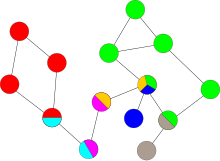
\includegraphics[width=0.8\textwidth]{Project/Details/Graph-Biconnected-Components.png} % Adjust width/height
              \caption{An example for Biconnected components in a graph}
              \label{fig:example}
          \end{figure}
          \begin{algorithm}[H]
              \caption{$simple\ cycles\ in\ a\ undirected\ graph$ (modified from algorithm 1)}
              \begin{algorithmic}
                  \State at line 1
                  \State \textbf{function} $\_all\_cycles\_iterator\_vertex(v, BCCs)$
                  \State \ldots
                  \State starting from line 8
                  \For{every neighbor $v' \in V$ of last vertex of $p$, such that $v'$ belong to the same biconnected component as $p$ in $BCCs$}
                  \State $p' \gets p + v'$
                  \If{$p'$ is simple path or simple cycle}
                  \State append $p'$ to the end of $queue$
                  \EndIf
                  \EndFor
                  \State \ldots
                  \State replaces lines 18 to 27
                  \State $BCCs \gets$ biconnected components of $D$
                  \State \ldots
                  \State at line 29
                  \For{$v \in S$}
                  \State add iterator \Call{$\_all\_cycles\_iterator\_vertex$}{$v, BCCs$} to $heap$
                  \EndFor
                  \State \ldots
              \end{algorithmic}
          \end{algorithm}
          This ensures that the shortest simple cycles are yielded without any drawbacks to efficiency compared to the method for directed graphs.

    \item \textbf{For weighted graphs}:
          the BFS finds shortest cycles first by searching by breadth,
          but for weighted graphs it cannot adapt
          to that since it never considers the weight and only considers
          the edges themselves. What I propose is adapting to a \href{https://en.wikipedia.org/wiki/Dijkstra's_algorithm}{Dijkstra}-like method,
          that is, by using a heap instead of a queue and storing
          and sorting based on the current path weight in the heap.
          This will ensure that the cycles with the smallest weight are retrieved first.
          \begin{algorithm}[H]
              \caption{$simple\ cycles\ in\ a\ weighted\ graph$ (modified from both algorithms 1 \& 2)}
              \begin{algorithmic}
                  \State \ldots
                  \State in $\_all\_cycles\_iterator\_vertex$
                  \State $heap \gets [(0,[v])]$ \Comment{a heap storing a path and its weight, while sorting on the weight}
                  \While{$heap$ not empty}
                  \State Extract $(w,p)$ from $heap$
                  \If{$p$ is a simple cycle}
                  \State \textbf{yield} $(w,p)$
                  \Else
                  \For{every neighbor $v' \in V$ of last vertex of $p$}
                  \State $p' \gets p + v'$
                  \State $w' \gets w + w(vv')$ \Comment{new weight of $p'$}
                  \If{$p'$ is simple path or simple cycle}
                  \State append $(w',p')$ to the $heap$
                  \EndIf
                  \EndFor
                  \EndIf
                  \EndWhile
                  \State \ldots
              \end{algorithmic}
          \end{algorithm}
\end{itemize}

\subparagraph{Deliverables}
These are the tasks that are expected to be delivered for this part of the
project.

\begin{itemize}
    \item Simple cycles in undirected graph
    \item Extend methods to support weighted graphs
\end{itemize}

Each and every task will contain the following

\begin{itemize}
    \item Core implementation
    \item Testing
    \item Documentation
\end{itemize}

All methods will follow a consistent input/output format:
\begin{itemize}
    \item \textbf{Input}: Parameters specifying cycle properties (e.g., length bounds, weight thresholds).
    \item \textbf{Output}: Iterators yielding cycles in ascending order of weight/length.
\end{itemize}




\subsubsection{K shortest simple paths}

\subparagraph{Current implementation}
The currently implemented methods are Yen's algorithm\cite{yen1971} and Feng's
algorithm (node classification)\cite{feng2014}. The method
$shortest\_simple\_paths$ will by default uses Yen's for undirected graphs and
Feng's for directed graphs.

\subparagraph{Proposed approaches}
To implement efficient algorithms for the k shortest simple paths problem, we
propose following the methods introduced in the paper “Finding the k Shortest
Simple Paths: Time and Space Trade-offs”\cite{kSSP2023}. This is a recent
paper, offering efficient optimizations for this problem. Furthermore, the fact
that David Coudert, the mentor of this GSoC project, is a co-author of the
paper makes this approach particularly well-suited for the project.

\subparagraph{Algorithms to be implemented}
\begin{itemize}
    \item \textbf{PNC} (Postponed Node Classification)\cite{kSSP2023}
          This algorithm performs well on graphs resembling road networks,
          where the structure tends to be sparse. It offer a faster performance in practice over the classic NC
          as It delays some of the calls until necessary, in order to avoid some of them.

          \begin{algorithm}[H]
              \caption{Postponed Node Classification (PNC)\cite{kSSP2023}}
              \begin{algorithmic}[1]
                  \Require A digraph \( D = (V, A) \), source \( s \in V \), sink \( t \in V \), integer \( k \)
                  \Ensure \( k \) shortest simple \( s-t \) paths

                  \State Let \( Candidate \gets \emptyset \) and \( Output \gets \emptyset \)
                  \State \( T \gets \) an SP in-branching of \( D \) rooted at \( t \)
                  \State Add \( (P_{st}(T), \omega(P_{st}(T)), 0, 1) \) to \( Candidate \)

                  \While{\( Candidate \neq \emptyset \) and \( |Output| < k \)}
                  \State \((P = (s, u_1, \cdots, t), \omega(P), i, \zeta) \gets \text{extract shortest element from } Candidate\)
                  \State \(\pi \gets (s, u_1, \cdots, u_{i-1})\)
                  \State \( Dev_{old} \gets \{e = (u_i, v) \mid \exists \text{ path in } Output \text{ with prefix } \pi.e \} \)

                  \If{\(\zeta = 1\) \textbf{(\( P \) is simple)}}
                  \State Add \( P \) to \( Output \)
                  \State \(\lambda \gets \text{vertex labeling of } D \text{ with respect to } P \text{ and } T\)

                  \For{each vertex \( u_j \) in \( (u_i, \cdots, t) \)}
                  \State \((u_j, v_{LB}) \gets \text{arc in } A \setminus Dev_{old} \text{ with min } \delta \text{ at } u_j\)
                  \State \( P_{LB} \gets (s, \cdots, u_j, v_{LB}, P^T_{v_{LB}t}) \)
                  \State \(\zeta' \gets 0\)
                  \If{\(\lambda(v_{LB}) > j\) \textbf{(\( P_{LB} \) is simple)}}
                  \State \(\zeta' \gets 1\)
                  \EndIf
                  \State Add \( (P_{LB}, \omega(P_{LB}), j, \zeta') \) to \( Candidate \)
                  \EndFor

                  \Else
                  \State Compute shortest \( u_i-t \) path \( Q \) in \( D' = (V \setminus \pi, A \setminus Dev_{old}) \)
                  \If{\( Q \) exists}
                  \State Add \( (P' = \pi.Q, \omega(P'), i, 1) \) to \( Candidate \)
                  \EndIf
                  \EndIf
                  \EndWhile

                  \State \Return \( Output \)
              \end{algorithmic}
          \end{algorithm}

    \item \textbf{PSB} (Parsimonious Sidetrack-Based)\cite{kSSP2023}
          This variant is significantly more efficient for complex networks
          (e.g., social networks, web graphs) where the degrees of the node is higher
          and diameter tends to be shorter. It offers a trade-off compared to the
          PNC as it uses more memory but is faster on this type of graphs.

          \begin{algorithm}[H]
              \caption{Sidetrack Based (SB) Algorithm for the \(k\)SSP (which the PSB is based upon)\cite{SB2016}}
              \begin{algorithmic}[1]
                  \Require A digraph \(D = (V, A)\), source \(s \in V\), sink \(t \in V\), integer \(k\)
                  \Ensure \(k\) shortest simple \(s\)-\(t\) paths

                  \State Let \(Candidate \gets \emptyset\) and \(Output \gets \emptyset\)
                  \State \(T_0 \gets\) an SP in-branching of \(D\) rooted at \(t\) containing \(s\)
                  \State Add \(\big((T_0), \omega(P_{st}(T_0)), \zeta = 1\big)\) to \(Candidate\)

                  \While{\(Candidate \neq \emptyset\) and \(|Output| < k\)}
                  \State \(\mu = \big(\varepsilon = ((T_0, e_0, \cdots, T_h, e_h = (u_h, v_h), T_{h+1}), lb, \zeta\big)) \gets\) a shortest element in \(Candidate\)

                  \If{\(\zeta = 1\)}
                  \State Extract \(\mu\) from \(Candidate\) and add \(\varepsilon\) to \(Output\)
                  \For{every deviation \(e = v_jv'\) with \(v_j \in P^{T_{h+1}}_{v_i,t}\)}
                  \State \(\varepsilon' \gets (T_0, e_0, \cdots, T_h, e_h, T_{h+1}, e, T_{h+1})\)
                  \State \(lb' \gets lb - \omega(P^{T_{h+1}}_{v_j,t}) + \omega(e) + \omega(P^{T_{h+1}}_{v't})\)
                  \If{\(\varepsilon'\) represents a simple path}
                  \State Add \(\mu' = (\varepsilon', lb', \zeta = 1)\) to \(Candidate\)
                  \Else
                  \State \(T' \gets\) the name of an SP in-branching of \(D_j(P)\) \Comment{\(T'\) is not computed yet}
                  \State Add \(\mu'' = \big(\varepsilon'' = (T_0, e_0, \cdots, T_h, e_h, T_{h+1}, e, T'), lb', \zeta = 0\big)\) to \(Candidate\)
                  \EndIf
                  \EndFor
                  \Else
                  \If{\(T_{h+1}\) has not been computed yet}
                  \State Compute \(T_{h+1}\), an SP in-branching of \(D_h(P)\)
                  \EndIf
                  \State \(\mu' = \big(\varepsilon' = (T_0, e_0, \cdots, T_h, e_h, T_{h+1}), lb + \omega(P^{T_{h+1}}_{v_i,t}) - \omega(P^{T_h}_{v_i,t}), \zeta = 1\big)\)
                  \State Add \(\mu'\) to \(Candidate\)
                  \EndIf
                  \EndWhile

                  \State \Return \(Output\)
              \end{algorithmic}
          \end{algorithm}
\end{itemize}

\subparagraph{Selection algorithm} As discussed in the paper, the optimal algorithm depends heavily on the
properties of the input graph. What I propose:

Analyzing the graph (e.g., average degree, diameter) and Automatically
selecting between PNC and PSB based on the graph’s properties:
\begin{itemize}
    \item Use PNC for sparse, road-like graphs
    \item Use PSB for dense, complex networks
\end{itemize}

\begin{figure}[ht]
    \centering

    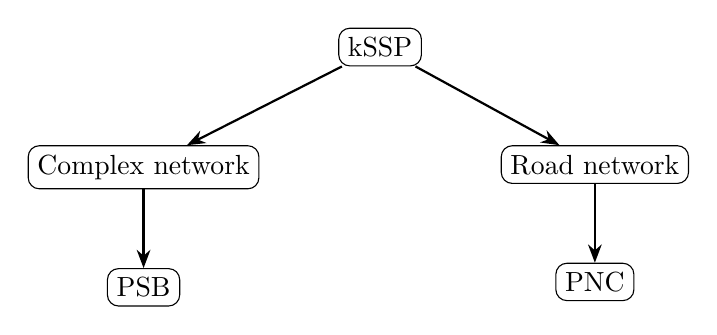
\begin{tikzpicture}
        [
        node distance=1cm and 1cm,
        every node/.style={draw, rectangle, rounded corners, align=center},
        arrow/.style={-{Stealth}, thick}
        ]

        \node (kssp) {kSSP};
        \node (complex) [below left=of kssp] {Complex network};
        \node (road) [below right=of kssp] {Road network};

        \node (psb) [below=of complex] {PSB};

        \node (pnc) [below=of road] {PNC};

        % Edges
        \draw [arrow] (kssp) -- (complex);
        \draw [arrow] (kssp) -- (road);

        \draw [arrow] (complex) -- (psb);

        \draw [arrow] (road) -- (pnc);

    \end{tikzpicture}
    \caption{Selection decisions for kSSP}
\end{figure}

Both algorithms natively support weighted directed graphs, and can be easily
extended to undirected graphs and unweighted graphs.

\subparagraph{Deliverables}
These are the tasks that are expected to be delivered for this part of the
project.

\begin{itemize}
    \item PNC (Postponed Node Classification)
    \item PSB (Parsimonious Sidetrack-Based)
    \item Selection algorithm
\end{itemize}

Each and every task will contain the following

\begin{itemize}
    \item Core implementation
    \item Testing
    \item Documentation
\end{itemize}

All methods will follow a consistent input/output format:
\begin{itemize}
    \item \textbf{Input}: Parameters specifying the paths properties (e.g., starting vertices, ending vertices, weight thresholds).
    \item \textbf{Output}: Iterators yielding paths in ascending order of weight/length.
\end{itemize}

\textbf{Note}: Neither the current implementation nor the proposed one will consider a
parameter k (the number of shortest paths to retrieve). Instead, the iterator
will continue computing paths until no more can be found.



% Schedule: A timetable, including special circumstances like exams or holidays, for the individual tasks.
\subsection{Schedule}

\begin{table}[H]
    \centering
    \footnotesize
    \begin{tabularx}{\textwidth}{|p{2.5cm}|p{2.5cm}|X|}
        \hline
        \textbf{Phase}                                                  & \textbf{Dates (Weeks)}            & \textbf{Activities} \\
        \hline
        Phase 1: Community Bonding \& Simple cycles in undirected graph & May 8 --- May 23 (3 wks)          &
        \begin{itemize}
            \item Engage with the community discuss project goals and details with the mentor.
            \item Familiarize myself more with the source code.
            \item Read the documentation and gain a deeper understanding of the development
                  process.
            \item Cycle enumeration: Simple cycles in undirected graphs
        \end{itemize}                                         \\
        \hline
        Phase 2: Extend methods to support weighted graphs              & May 24 --- June 07 (2 wks)        &
        \begin{itemize}
            \item Cycle enumeration: Extend methods to support weighted graphs
            \item Extra testing for Cycle enumeration part.
        \end{itemize}                                                         \\
        \hline
        Phase 3: PNC                                                    & June 08 --- July 13 (4 wks)       &
        \begin{itemize}
            \item kSSP: PNC (Postponed Node Classification)
        \end{itemize}                                                                            \\
        \hline
        Phase 4: PSB                                                    & July 14 --- August 11 (4 wks)     &
        \begin{itemize}
            \item kSSP: PSB (Parsimonious Sidetrack-Based)
        \end{itemize}                                                                             \\
        \hline
        Phase 5: Selection algorithm \& Finalization                    & August 12 --- September 1 (3 wks) &
        \begin{itemize}
            \item kSSP: Selection algorithm.
            \item Extra Testing for kSSP part.
            \item Address any remaining issues or bugs.
            \item Finalization.
        \end{itemize}                                                                                \\
        \hline
    \end{tabularx}
    \caption{Project Plan and Timeline.}
\end{table}

\begin{itemize}
    \item Every phase is tested and documented before proceeding to the next phase.
    \item My availability every week ranges from 20 to 25 hours.
    \item I will have my final exams and some holidays in late May / early June. Although
          this will not affect the project schedule, I will be unavailable on certain
          days.
    \item Full-Time Job Possibility: There is a chance that I could start a full-time job
          around mid-July or August. Regardless of this, I will ensure that the project
          schedule is met and all planned milestones are completed on time.
\end{itemize}



% Risk Management: 
% Try to anticipate potential problems and explain, 
% how to mitigate them. 
% Propose alternative scenarios,
% if a particular milestone isn't reached, 
% to still successfully complete the project.

\subsection{Risk Management}
While I believe I am well-suited for this project, I have identified several
potential risks that could impact the project:

\begin{enumerate}
  \item Some parts of this project depend on modules that are already implemented (like
        trees and other data structures). I might face problems with these modules,
        such as bugs or unexpected behavior. In the best case, I will be able to fix
        the issues in these modules and continue with the project as planned. In the
        worst case, I will write a temporary implementation to replace the broken
        module. This might cause some code duplication, but it will let me continue
        working until the original module is fixed.

  \item Delays might happen due to either unexpected bugs or limitations. When drafting
        the project schedule, I made sure to give extra time for each phase. However,
        in worst case scenario, the order of the phases in the schedule guarantees that
        a big part of the project will be done.

\end{enumerate}

\clearpage
\bibliographystyle{plain}
\bibliography{ref}

\end{document}
